\documentclass[preprint,11pt,3p]{article}

\usepackage{tocloft}
\usepackage{color}
\usepackage{hyperref}
\usepackage{graphicx}
\usepackage{float}
\usepackage{subcaption}
\usepackage{amsmath} 
\usepackage{tikz} 
\usepackage{epigraph}
\usepackage{lipsum} 
\usepackage{indentfirst}


\renewcommand\epigraphflush{flushright}
\renewcommand\epigraphsize{\normalsize}
\setlength\epigraphwidth{0.7\textwidth}
\renewcommand{\abstractname}{Executive Summary}

\definecolor{titlepagecolor}{cmyk}{1,.60,0,.40}

\DeclareFixedFont{\titlefont}{T1}{ppl}{b}{it}{0.5in}

\makeatletter                       
\def\printauthor{%                  
    {\large \@author}}              
\makeatother
\author{%
    Eric Altenburg \\
    \texttt{ealtenbu@stevens.edu}\vspace{20pt} \\
    Michael McCreesh \\
    \texttt{mmccree1@stevens.edu}\vspace{20pt} \\
    Hamzah Nizami \\
    \texttt{hnizami1@stevens.edu}\vspace{20pt} \\
    Constance Xu \\
    \texttt{cxu16@stevens.edu}
    }

% The following code is borrowed from: https://tex.stackexchange.com/a/86310/10898

\newcommand\titlepagedecoration{%
\begin{tikzpicture}[remember picture,overlay,shorten >= -10pt]

\coordinate (aux1) at ([yshift=-15pt]current page.north east);
\coordinate (aux2) at ([yshift=-410pt]current page.north east);
\coordinate (aux3) at ([xshift=-4.5cm]current page.north east);
\coordinate (aux4) at ([yshift=-150pt]current page.north east);

\begin{scope}[titlepagecolor!40,line width=12pt,rounded corners=12pt]
\draw
  (aux1) -- coordinate (a)
  ++(225:5) --
  ++(-45:5.1) coordinate (b);
\draw[shorten <= -10pt]
  (aux3) --
  (a) --
  (aux1);
\draw[opacity=0.6,titlepagecolor,shorten <= -10pt]
  (b) --
  ++(225:2.2) --
  ++(-45:2.2);
\end{scope}
\draw[titlepagecolor,line width=8pt,rounded corners=8pt,shorten <= -10pt]
  (aux4) --
  ++(225:0.8) --
  ++(-45:0.8);
\begin{scope}[titlepagecolor!70,line width=6pt,rounded corners=8pt]
\draw[shorten <= -10pt]
  (aux2) --
  ++(225:3) coordinate[pos=0.45] (c) --
  ++(-45:3.1);
\draw
  (aux2) --
  (c) --
  ++(135:2.5) --
  ++(45:2.5) --
  ++(-45:2.5) coordinate[pos=0.3] (d);   
\draw 
  (d) -- +(45:1);
\end{scope}
\end{tikzpicture}%
}

\begin{document}
\begin{titlepage}

\noindent
\titlefont Cruise Control Software Development Version 0.07\par
\epigraph{We pledge our honor that we have abided by the Stevens Honor System.}%
{\textit{CS347: Software Development Processes |  Spring 2020}\\ \textsc{Team Mike}}
\null\vfill
\vspace*{1cm}
\noindent
\hfill
\begin{minipage}{0.35\linewidth}
    \begin{flushright}
        \printauthor
    \end{flushright}
\end{minipage}
%
\begin{minipage}{0.02\linewidth}
    \rule{1pt}{125pt}
\end{minipage}
\titlepagedecoration
\end{titlepage}




\newpage

\tableofcontents
\newpage

\section{Executive Summary}
Team Mike is a startup initiative aimed at solving problems that come to light as
society begins to adopt new technologies. One of which pertains to autonomous
driving and “smart cars” as they are beginning to break into the automobile
market more and more every year with examples such as Tesla and Ford. In a
perfect world, if every driving car were to be a smart car with “autopilot,” then
it would make sense for each of them to communicate cruise control data with
each other to reduce traffic build-up and make traveling more efficient. Through
rotational leadership on a monthly basis, each team member possesses a set of
distinct skills that can translate to highly efficient work sessions. Aside from
developing a traditional cruise control, the aim is to make the software open source as it will serve as the foundation to a more interconnected logistical future in which autonomous cars can fully achieve
their potential within a growing technologically advanced society. 
\newpage

\section {Introduction}
The past century has seen an explosion of innovation on a scale never before seen
in human history. The rapid development and refinement of a myriad of motor
technologies catalyzed the innovation process by allowing ideas to transfer at
rates never before seen. With the constraint of distance loosening thanks to
every iteration of the automobile, people have been granted more freedom to
do what they please. While the automobile has enhanced society in several
ways, there are some glaring problems that need to be addressed to continue
the current rate of human progress and innovation. One of the biggest problems
is driver fatigue, which is responsible for approximately 72,000 crashes annually.
Programming the automobile to be reliably autonomous to a degree is one way
to circumvent the issue of driver fatigue and making roads safer. That’s exactly
what cruise control aims to do. By moderating the speed of the vehicle by itself,
cruise controls aim to lessen the effects of driver fatigue on the road. However,
the technology is not perfect, and Team Mike aims to resolve that by creating
the perfect cruise control system. \par
When it was implemented in 1958, cruise control was suitable for that era,
however, as technology continually improves, the embedded software must as
well. For longer car trips, it does not make sense for users to constantly accelerate
and decelerate for several miles; this is where cruise control comes in. By being
able to set the speed, the user is now able to accurately set and maintain the
speed they wish to without having to constantly intervene which, over time,
would cause less harm to the vehicle as variable speed and RPMs are not as
desirable as that of near-constant. \par
Our group intends to use an Agile method to implement our version of cruise
control. This would encourage code sprints in two-week lengths where work
will be divided into smaller sections and distributed based on each members’
strengths. The Agile method may vary as to which one we specifically choose
but regardless, this project will not come to fruition using Waterfall or other
methods. The way that we are going to organize our group is through weekly
meetings and ensuring that everyone knows their tasks for the week. These
weekly meetings can also serve as a place where team members mention any
obstacles that have come in their way when trying to resolve a problem, and
also serve as a time where the team as a collective can try to think of solutions
around those obstacles. We also plan on giving real-time updates about any
progress made through Slack in order to ensure all members of the team are
equipped with the most recent developments of the project. We also intend on
using Java or C++ to implement our cruise control system. We believe that the
high-performance Java provides and the fact that its part of the Object-Oriented
Programming (OOP) paradigm makes it perfect for embedded systems. \par
There are a plethora of features that make up cruise control. As most cruise
controls are seen on vehicles, there are generally a few buttons: increase speed
(and sometimes decrease speed) and the button that starts cruise control. Once
cruise control is set, the user then has the ability to increase, decrease, or
maintain the speed of a vehicle. Furthermore, if the user presses on the brake,
then cruise control is automatically deactivated. The system also allows for the
operator of a vehicle to manually deactivate it. \par
To successfully implement the features of maintaining a steady speed and a
safe distance away from other cars, there are certain requirements to fulfill. At a
high level, proper hardware with fast, reliable sensors is critical for this project.
Furthermore, lives are fundamentally dependent on this product and therefore
it requires software that is error-resistant and thus a strong development and
QA (quality assurance) team. In addition, the software must also perform it’s
expected tasks of moderating speed, maintaining a safe distance and switching
back control to the driver when prompted to quickly. Having a cruise control
software that is slow would be ineffective, so speed and accuracy are critical
requirements for the software as well as the hardware. This is a mission-critical
system because if it were to fail, it would put the lives of people in danger.

\newpage
\section{Requirements}

\subsection{Input}
\begin{enumerate}
	\item The system shall accept electric power from the alternator.
	\item The power button that allows for the state of the system to change from on to off or vice versa.
	\item When pressed, a button will either accelerate or decelerate in 1 mph increments. 
	\item When the brake is pressed, the cruise control system will unset the speed and give control back to the user until the user specifies a new speed to be set.
	\item If the entire car turns off, then a signal will be sent to turn off the cruise control system.
	\item RPM (Rotations Per Minute) sensor should be connected to the front axle and able to take readings for accurate speed calculations. 
	% \item RADAR sensor must be able to detect nearby vehicles/obstacles to avoid collision. %Do we really wanna do this
	\item Engine sensor must be able to take input from the engine to tell the cruise control system to turn on or off.
		\begin{enumerate}
			\item If the engine is turned on, the cruise control system must be ready for use within 3 seconds of the engine being turned on.
		\end{enumerate}
	\item If the gas pedal is pressed, the vehicle will continue to accelerate at the control of the user, but when the gas pedal is released the cruise control system will continue to the previously set speed.
	% \item Brake pedal sensor must be able to take input from user to stop when pressed and keep going when released.
\end{enumerate}

\subsection{Output}
\begin{enumerate}
	\item Keep a log of activity in the system files to help debug in the event of a malfunction.
	\item For every speed increase made by the user in the cruise control system, a visual indication by the software is necessary. This is so that the user minimizes their own human error. So, every time you increase the speed, you can see the cruise control speed on the car menu increasing by however much the user wants it to.
	\item The system displays successful activation or deactivation in 10 milliseconds. 
		\begin{enumerate}
			\item Numbers are subject to change depending on how inputs are received from surrounding system, but are expected to be in around that same ballpark.
		\end{enumerate}
	\item Keep a log of every time the cruise control system is used and at what speed written to the system files.
	% \item This module must be able to do what the user wants within a fast time frame, less than ten milliseconds. *Numbers are subject to change depending on how inputs are received from surrounding system, but are expected to be in around that same ballpark.*
	\item Once the cruise control system is turned on, it must be readily available. The engine sensor must be able to understand that the engine is on and tell the cruise control system that, if the user so wishes, it must activate. 
	\item With all the inputs it is taking from all the sensors, the software must be able to deliver the desired output for each function in less than 15 milliseconds. 
		\begin{enumerate}
			\item The brake pedal sensor must be able to tell the software that the user has stopped, and stop the cruise control system. *Numbers are subject to change depending on how inputs are received from surrounding system, but are expected to be in around that same ballpark.*
		\end{enumerate}
\end{enumerate}

\subsection{Functional}
\begin{enumerate}
	\item The system shall accept direct current from the car battery to support logging after engine shut down.
	\item The system shall receive the time and date from the car's clock every second.
	\item A physical will be provided by the system for technicians to access the unit.
	\item Hardware shall have a 4 nine (99.99\%) availability.
	\item Software shall have a 5 nine (99.999\%) availability.
	\item While the cruise control system is on and a speed is set, it must be able to increase and decrease the speed by 1 mph.
	\item Able to switch the cruise control system on or off provided the engine is on.
	\item Interpret engine on and off signal to allow for the cruise control system to be turned on within 3 seconds of received the signal.
	\item Only allow the cruise control system to be activated when at a minimum speed of 25 mph. 
		\begin{enumerate}
			\item If the speed is set to 25 mph, the user cannot decrease the speed below 25 mph.
		\end{enumerate} %What if we set speed and and set speed below this
	\item Maximum speed that cruise control system can be set to is at 125 mph.
	\item While the cruise control system is on, if a user is driving at a speed of at least 25 mph and decides to set the speed, the cruise control system will maintain that speed.
	\item If the user presses and continues to press the brakes, the user will not be able to set the speed.
	\item If the user presses and continues to press the gas pedal, the user can set the current speed for the cruise control system, but it will immediately pause as stated in the input requirements then resume after the user releases the gas pedal.
\end{enumerate}

\subsection{Security}
\begin{enumerate}
	\item No external interface to reduce potential tampering. This applies to both the hardware such as sensors and the general cruise control system software. There would be no easy access to the cruise control system hardware or software so that the likelihood of someone being able to create issues is reduced substantially. 
	\item No Internet or Bluetooth connection. This is so that no bad actors can meddle with the car's system and hence, keeps the drivers safer as cyber security becomes more of an issue.
	\item An administrator will need hardware to make changes to the mechanisms. The administrator must be authorized to make these changes and they must be a trusted third party or those who created the cruise control system themselves. 
\end{enumerate}

\section{Requirements Analysis Model}

\subsection{UML Use Cases \& Diagram} 
See Figure ~\ref{fig:ccUML1} for general use cases of cruise control system.
	\begin{figure}[H]
		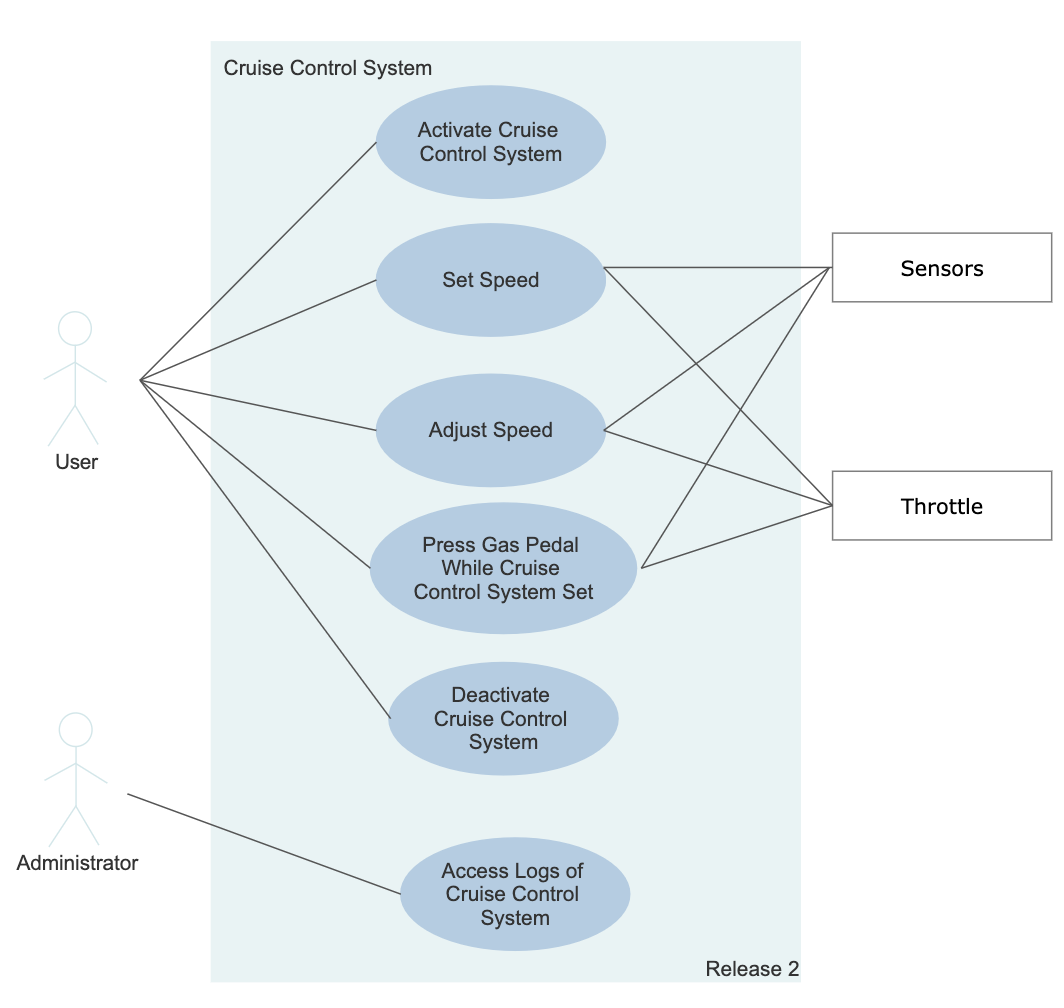
\includegraphics[width=0.9\textwidth]{images/ccUseCaseUML.png}
		\caption{Sample UML diagram for cruise control system use cases.}
		\label{fig:ccUML1}
	\end{figure}

It should be mentioned that there are two similar sounding states that need to be clarified:
\begin{itemize}
	\item Activated
		\begin{itemize}
			\item Granted the vehicle is on, the cruise control system is also now waiting for the speed to be set by the user.
		\end{itemize}
	\item Set/Unset
		\begin{itemize}
			\item Given that the cruise control system has been \textbf{activated}, the user has requested for the speed to be maintained at its current speed.
			\item Given that the cruise control system has been \textbf{activated} and the cruise control system is in the \textbf{set} state, the user can either press the brake or press a button to unset the speed and revert back to the \textbf{activated} state.
		\end{itemize}
\end{itemize}
\begin{enumerate}
	\item Use Case 1: User activates the cruise control system
		\begin{enumerate}
			\item Given that the vehicle is on, the user requests an activation of the cruise control system.
			\item Cruise control system activates.
			\item The cruise control system provides a visual feedback that it has been activated.
		\end{enumerate}
	\item Use Case 2: User sets the speed
		\begin{enumerate}
			\item Given that the vehicle is on and the cruise control system is in the activated state, the system requests values from sensors.
			\item Sensors provide values for approval to set cruise control system at current speed.
			\item Cruise control system requests the Engine Management System (EMS) set the speed at current position.
			\item EMS Speed (Throttle) is set at current speed.
			\item Cruise control system provides visual feedback to the user that the cruise control is set and working.
			\item Sensors provide the changing environmental information to the cruise control unit (such as speed, request for increase/decrease speed, and brake).
			\item Cruise control system detects the changes from the sensors and request adjusting speed or deactivating Cruise Control system accordingly.
			\item Speed (Throttle) position is continuously set to new values to ensure that the speed remains constant.
			\item Speed is continuously reported to the cruise control system.
		\end{enumerate}
	\item Use Case 3: User adjusts speed
		\begin{enumerate}
			\item If the cruise control system is in the set state, the user requests an adjustment of cruise control system speed.
			\item Cruise control system provides visual feedback that the system will alter the speed of the vehicle.
			\item Cruise control system slowly adjusts the speed of the vehicle to match that of the request.
			\item When the desired speed is reached, the cruise control system will provide visual feedback that the adjustment has been completed.
		\end{enumerate}
	\item Use Case 4: User presses gas pedal while the cruise control system is set
		\begin{enumerate}
			\item If the cruise control system is in the set state, the user presses on the gas pedal.
			\item In the event that the vehicle accelerates, the cruise control system will continually request the EMS to be set to the previously specified speed.
			\item Speed will be continuously reported to the cruise control system.
			\item After the user releases the gas pedal and the vehicle stops accelerating, the cruise control system will request for the EMS to be set to the previous specified speed.
			\item The vehicle will naturally decelerate nearing the old set speed, and once reached, the cruise control system will resume with the set speed.
		\end{enumerate}
	\item Use Case 5: User deactivates cruise control system
		\begin{enumerate}
			\item If the cruise control system is activated, the user requests a deactivation of the cruise control system.
			\item Cruise control system deactivates.
			\item Cruise control system provides visual feedback that it has been deactivated.
		\end{enumerate}
	\item Use Case 6: Technician accesses logs of cruise control system
		\begin{enumerate}
			\item With the vehicle turned on and the cruise control activated, an administrator will have to use a proprietary physical hardware key in order to gain root access.
			\item Once access has been granted, the administrator can download the logs to an external storage device through a USB port.
			\item Once downloaded, the administrator must log out using the same proprietary physical hardware key.
		\end{enumerate}
\end{enumerate}

\subsection{UML Class-Based Modeling}
\begin{enumerate}
	\item See Figure ~\ref{fig:classUML} for the class-based modeling for the cruise control system.
		\begin{figure}[H]
			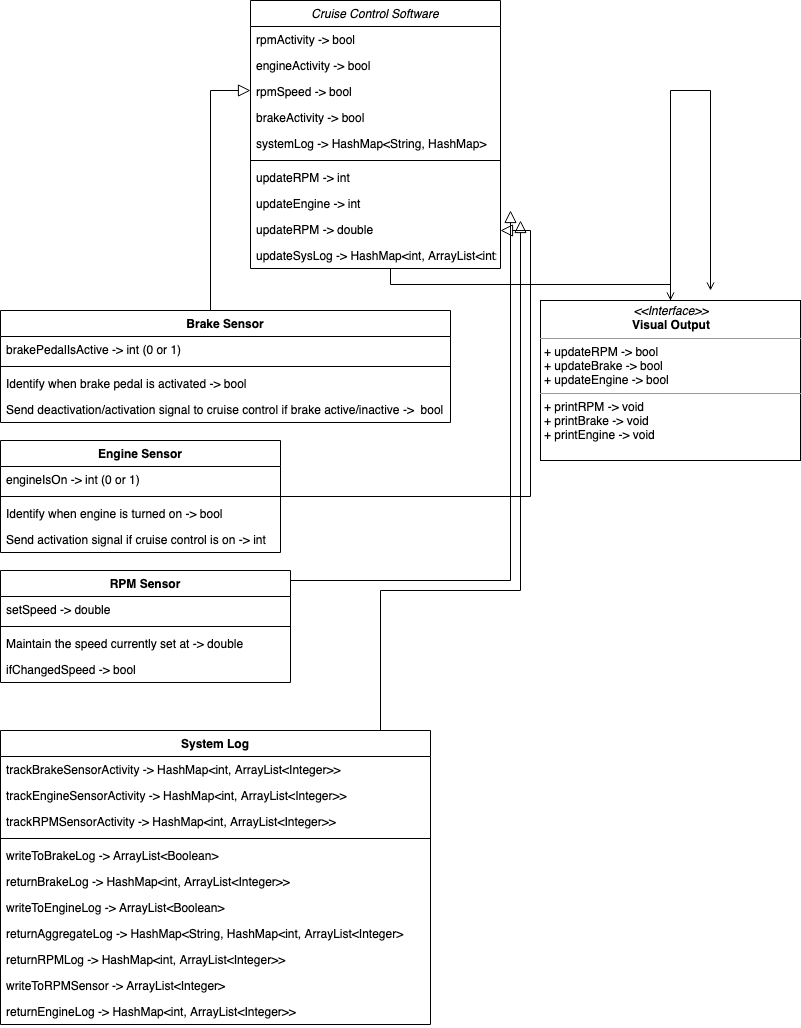
\includegraphics[width=0.9\textwidth]{images/classUML.png}
			\caption{Sample UML class-based model for the cruise control system.}
			\label{fig:classUML}
		\end{figure}
\end{enumerate}

\subsection{UML CRC Model Index Card}
\begin{enumerate}
	\item See Figure ~\ref{fig:indexUML} for the CRC Model Index Cards for the cruise control system.
		\begin{figure}[H]
			\begin{subfigure}{.3\textwidth}
				\centering
				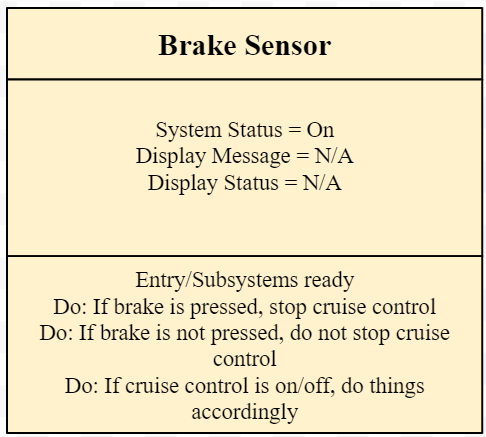
\includegraphics[width=.8\linewidth]{images/brakesensorindex.PNG}
				\label{fig:sub1}
			\end{subfigure}
			\begin{subfigure}{.3\textwidth}
				\centering
				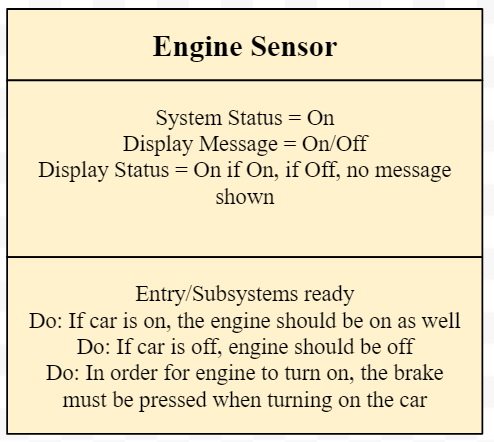
\includegraphics[width=.8\linewidth]{images/enginesensorindex.PNG}
				\label{fig:sub2}
			\end{subfigure}
			\begin{subfigure}{.3\textwidth}
				\centering
				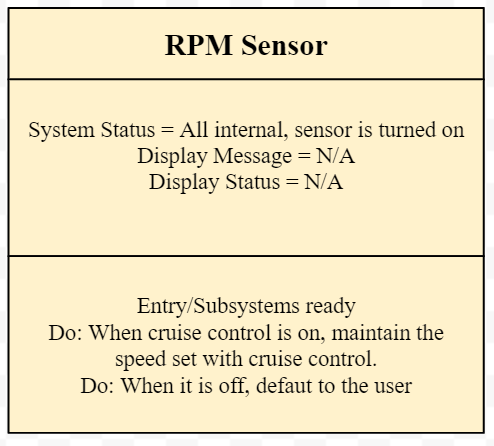
\includegraphics[width=.8\linewidth]{images/rpmsensorindex.PNG}
				\label{fig:sub3}
			\end{subfigure}
			\center
			\begin{subfigure}{.3\textwidth}
				\centering
				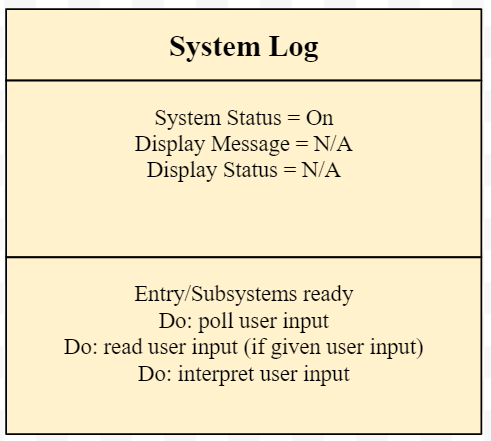
\includegraphics[width=.8\linewidth]{images/systemlogindex.PNG}
				\label{fig:sub3}
			\end{subfigure}
			\begin{subfigure}{.3\textwidth}
				\centering
				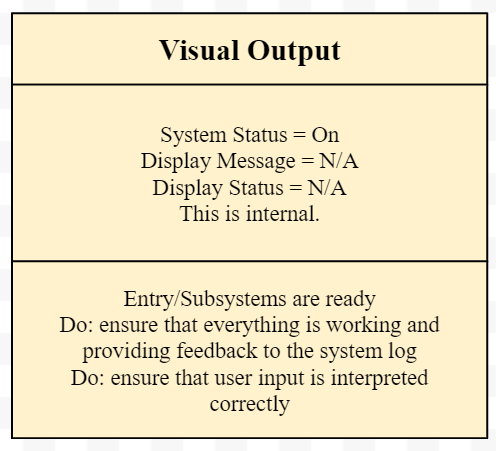
\includegraphics[width=.8\linewidth]{images/visualoutputindex.PNG}
				\label{fig:sub3}
			\end{subfigure}
			\caption{Sample UML CRC model index cards for the cruise control system.}
			\label{fig:indexUML}
		\end{figure}
\end{enumerate}

\subsection{UML Activity Diagram}
\begin{enumerate}
	\item See Figure ~\ref{fig:activityUML} for the activity diagram of the cruise control system.
		\begin{figure}[H]
			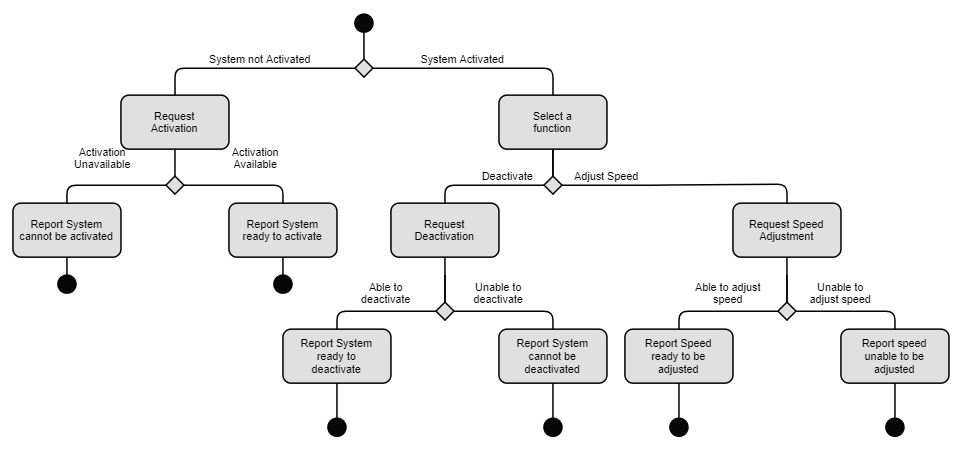
\includegraphics[width=0.9\textwidth]{images/activityUML.jpg}
			\caption{Sample UML activity diagram for the cruise control system.}
			\label{fig:activityUML}
		\end{figure} 
\end{enumerate}

\subsection{UML Sequence Diagram}
\begin{enumerate}
	\item See Figure ~\ref{fig:ccActivation} for sequence diagram of the activation of the cruise control system.
		\begin{figure}[H]
			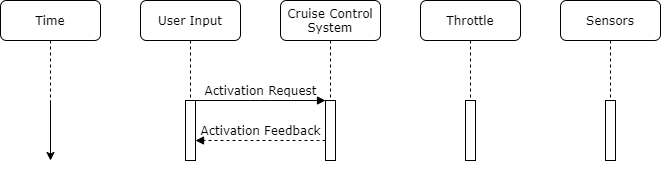
\includegraphics[width=0.9\textwidth]{images/activation.png}
			\caption{Sequence UML digram for activation of the cruise control system.}
			\label{fig:ccActivation}
		\end{figure}
	\item See Figure ~\ref{fig:ccSet} for sequence diagram of cruise control system setting speed.
		\begin{figure}[H]
			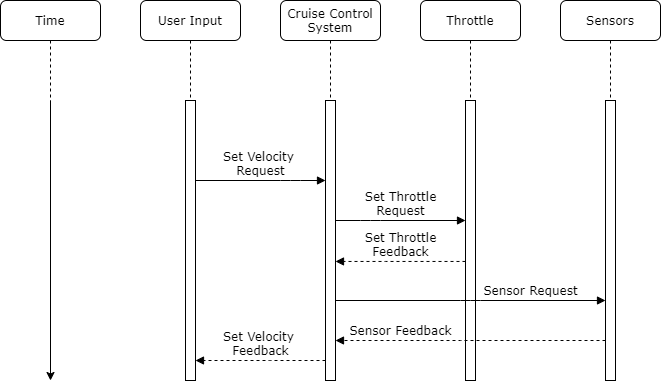
\includegraphics[width=0.9\textwidth]{images/set.png}
			\caption{Sequence UML diagram for the cruise control system setting speed.}
			\label{fig:ccSet}
		\end{figure}
	\item See Figure ~\ref{fig:ccAdjust} for sequence diagram of cruise control system adjusting speed.
		\begin{figure}[H]
			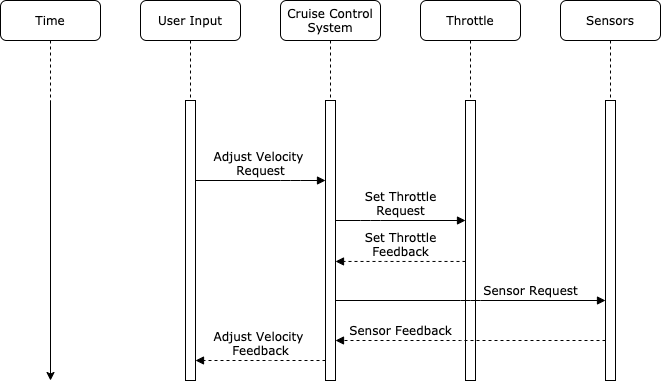
\includegraphics[width=0.9\textwidth]{images/adjustSequence.png}
			\caption{Sequence UML diagram for the cruise control system adjusting speed.}
			\label{fig:ccAdjust}
		\end{figure}
	\item See Figure ~\ref{fig:ccGas} for sequence diagram of the cruise control system being suspended when the user presses the gas pedal.
		\begin{figure}[H]
			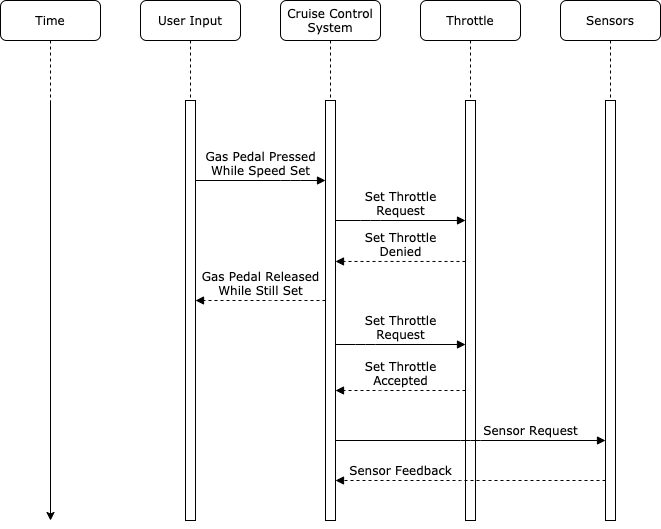
\includegraphics[width=0.9\textwidth]{images/gasPedalPressedSequence.png}
			\caption{Sequence UML diagram for the cruise control system suspending during gas pedal being pressed.}
			\label{fig:ccGas}
		\end{figure}
	\item See Figure ~\ref{fig:ccDeactivate} for sequence diagram of the cruise control system being deactivated.
		\begin{figure}[H]
			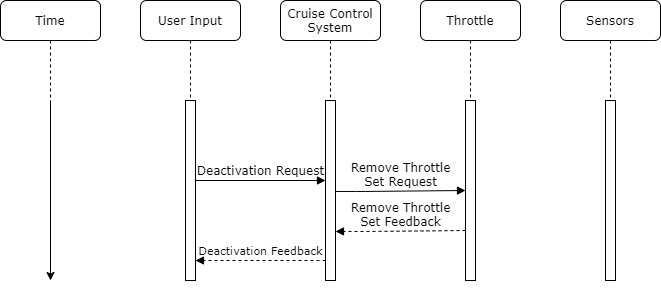
\includegraphics[width=0.9\textwidth]{images/deactivation.png}
			\caption{Sequence UML diagram for the cruise control system being deactivated.}
			\label{fig:ccDeactivate}
		\end{figure}
	\item See Figure ~\ref{fig:ccAdmin} for sequence diagram of the administrator accessing the cruise control system logs.
		\begin{figure}[H]
			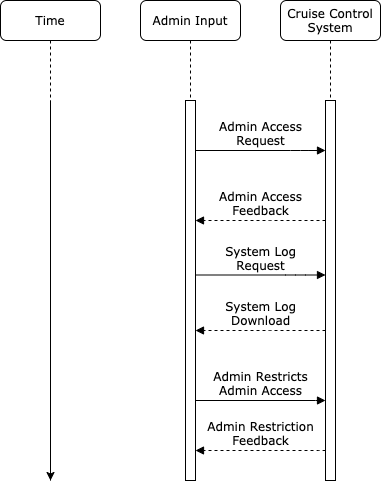
\includegraphics[width=0.9\textwidth]{images/sequenceAdmin.png}
			\caption{Sequence UML diagram for the administrator accessing cruise control system logs.}
			\label{fig:ccAdmin}
		\end{figure}
\end{enumerate}

\subsection{UML State Diagram}
\begin{enumerate}
	\item See Figure ~\ref{fig:stateUML} for the state diagram of the cruise control system.
			\begin{figure}[H]
				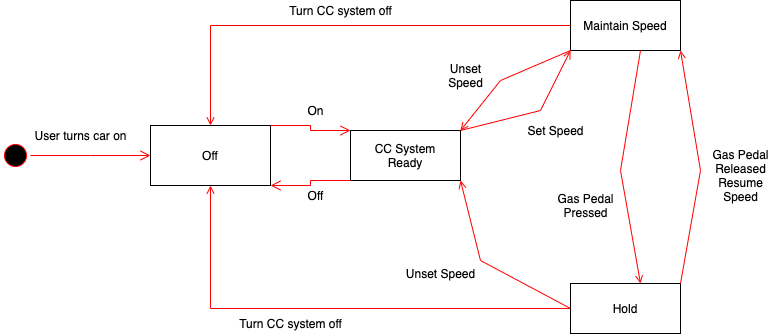
\includegraphics[width=0.9\textwidth]{images/stateUML.png}
				\caption{Sample UML state diagram for the cruise control system.}
				\label{fig:stateUML}
			\end{figure}
\end{enumerate}

\section{Software Architecture}

\subsection{Architecture Style} 
\subsection{Components} 
\subsection{Control Management} 
\subsection{Data Architecture} 
In terms of data architecture, the plan is to adopt a scalable, object-oriented, NoSQL database like MongoDB. Considering that the project is going to be programmed in an object oriented language such as Java or C++, having the data schema represented in the same programming paradigm streamlines the technical thought process behind the project. Furthermore, MongoDB is known for its high availability and performance. Having a data schema known for reliability is imperative for a mission critical piece of software like cruise control.\par
Due to the use of Java/C++ and MongoDB, the general paradigm of the data architecture is object-oriented. We will also be using a call and return architecture in conjunction, which will be discussed later on in the document.  An object-oriented data architecture means that the components of a system encapsulate data and the operations that must be applied to manipulate the data. Communication between the components is done via message passing. Due to the object-oriented nature of the system, that means that the data between components is communicated via synchronous message-passing. Message passing is a critical since it relies on all the components to be active in order to pass information. This makes it easier to identify when the system is down. This also means that data objects are passed around the system based on need. \par
The mode of data transfer is direct memory access. Since data components exist in this cruise control (such as a data component for RPM sensors, one for brake sensors, one for engine sensors, one for system logs), each component can access each other if they need. So, if a system log needs to be generated, it can access RPM sensors, brake sensors and engine sensors data directly and then compile and create the log files. Thanks to this direct access model, functional components interact with data components directly as well. For example, the visual interface can simply query the RPM sensor object to obtain the information needed about speed. There are no proxies or extra steps needed, thus avoiding the chance of dependency issues. This is where the call-and-return architecture comes in. If a functional component needs to access something, a subprocess can run to access the needed data without deterring the general flow more mission-critical pieces of the software. \par 
As we can see, the control of the program sets up the relationship between itself and the data on a need by need basis. Whenever the program needs something, it can directly access the data object to store, modify or delete values. 

\subsection{Architectural Designs} 
\begin{enumerate}
	\item See Figure ~\ref{fig:context} for the architecture context diagram.
		\begin{figure}[H]
			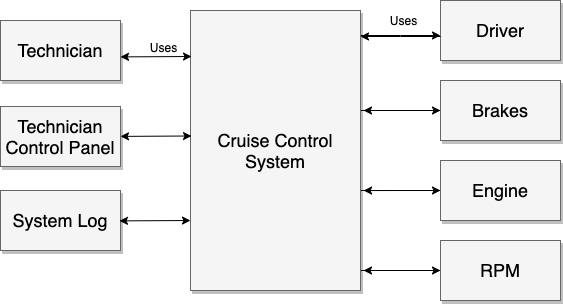
\includegraphics[width=0.9\textwidth]{images/Architectural_Context_Diagram.png}
			\caption{context diagram}
			\label{fig:context}
		\end{figure}
	\item Cruise control archetypes
		\begin{enumerate}
			\item System logging
				\begin{figure}[H]
					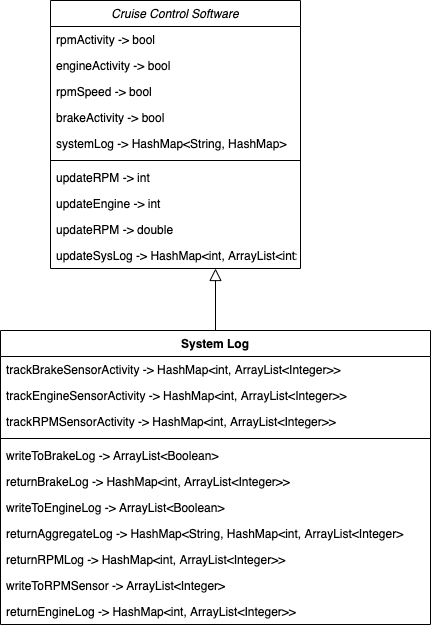
\includegraphics[width=0.9\textwidth]{images/classMapCS347_logging.png}
					\caption{System logging}
					\label{fig:logging}
				\end{figure}
			\item Set, maintain, and change speed
				\begin{figure}[H]
					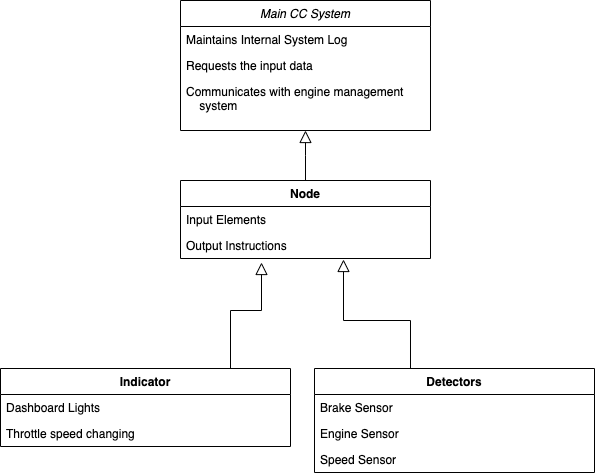
\includegraphics[width=0.9\textwidth]{images/classMapCS347_set.png}
					\caption{Set, maintain, and change speed}
					\label{fig:set}
				\end{figure}
			\item Visual output
				\begin{figure}[H]
					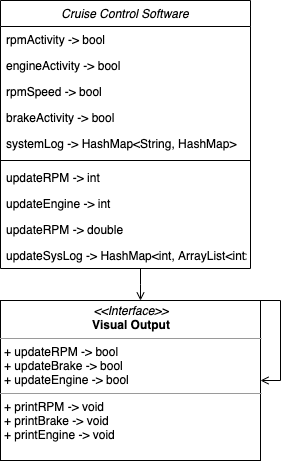
\includegraphics[width=0.9\textwidth]{images/classMapCS347_visual_output.png}
					\caption{Visual output}
					\label{fig:visual}
				\end{figure}
		\end{enumerate}
	\item See Figure ~\ref{fig:top} for the cruise control Top-Level component
		\begin{figure}[H]
			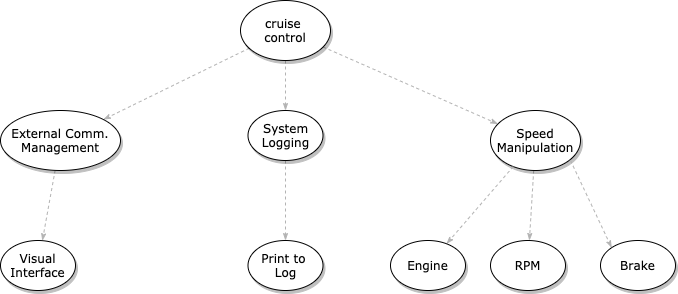
\includegraphics[width=0.9\textwidth]{images/architecture_top_level.png}
			\caption{Top-level component}
			\label{fig:top}
		\end{figure}
	\item See Figure ~\ref{fig:refined} for the refined component architecture
		\begin{figure}[H]
			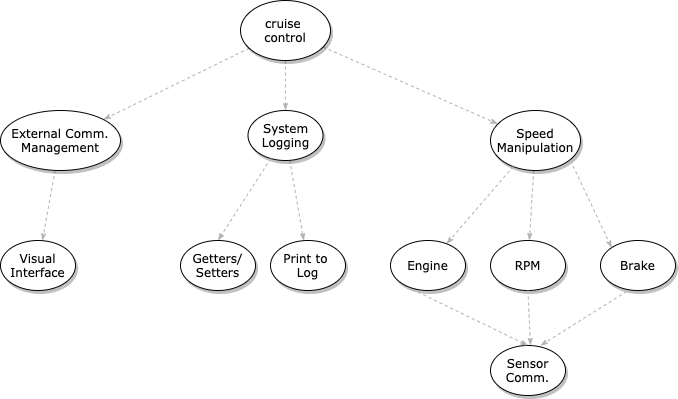
\includegraphics[width=0.9\textwidth]{images/architecture_refined_component.png}
			\caption{Refined component}
			\label{fig:refined}
		\end{figure}
\end{enumerate}

\subsection{Issues}

\end{document}

